% ****** Start of file aipsamp.tex ******
%
%   This file is part of the AIP files in the AIP distribution for REVTeX 4.
%   Version 4.1 of REVTeX, October 2009
%
%   Copyright (c) 2009 American Institute of Physics.
%
%   See the AIP README file for restrictions and more information.
%
% TeX'ing this file requires that you have AMS-LaTeX 2.0 installed
% as well as the rest of the prerequisites for REVTeX 4.1
%
% It also requires running BibTeX. The commands are as follows:
%
%  1)  latex  aipsamp
%  2)  bibtex aipsamp
%  3)  latex  aipsamp
%  4)  latex  aipsamp
%
% Use this file as a source of example code for your aip document.
% Use the file aiptemplate.tex as a template for your document.
\documentclass[%
aps,
pra,%
amsmath,amssymb,
preprint,%
reprint,%
notitlepage,
a4paper]{revtex4-1}
\usepackage{natbib}
\usepackage[utf8]{inputenc}
\usepackage{graphicx}% Include figure files
\usepackage{dcolumn}% Align table columns on decimal point
\usepackage{bm}% bold math
\usepackage[mathlines]{lineno}% Enable numbering of text and display math
%\linenumbers\relax % Commence numbering lines
\usepackage[spanish, english]{babel}
\usepackage{float}
\usepackage{rotating}
\usepackage{afterpage}
\usepackage{capt-of}
\usepackage{hyperref}
\usepackage{mathtools}
\usepackage{physics}
\usepackage[separate-uncertainty=true]{siunitx}
%\bibliographystyle{apsrev4-1}
%\usepackage{doi}
\bibliographystyle{aipauth4-1}
\newcommand{\md}{\texttt{md1} }
\newcommand{\average}[1]{\langle #1 \rangle}


\begin{document}
	
	%\preprint{AIP/123-QED}
	
	\title[Computer Simulation of Physical Systems]{Molecular Dynamics of Liquid Argon}% Force line breaks with \\
	
	\author{Daniel Felipe Forero Sánchez}
	%Lines break automatically or can be forced with \\
	
	
	\date{\today}% It is always \today, today,
	%  but any date may be explicitly specified
		%display desired

	
	\begin{abstract}
		

	\end{abstract}


	\maketitle

	
	\section{Introduction}
	Molecular dynamics simulations have been fundamental tools in science since they allow for the detailed analysis of various properties of the system that are impossible to probe experimentally. However, to properly simulate a physical system is a complex problem on its own, owing to the size of such systems. Molecular dynamics treats the system as a collection of particles evolving according to the Lennard-Jones potential \cite{Jones1924}, so it can be then regarded as a simulation from ``first principles''. To track the position and velocities of $10^{23}$ particles is, in practice, impossible. In such a limit one often uses emergent models such as fluid dynamics. Nonetheless, it is possible to properly model a small physical system with MD and make it an accurate reproduction of the real world \cite{Rahman1964}.\\
	On the other hand, it is also possible to simulate a system by walking or sampling the phase space following the canonical probability distribution. This can be accomplished though a Monte Carlo (MC) simulation.\\
	In the present work we set to characterize a fluid system through some physical quantities introduced in section \ref{sec:theory}. We describe the methods used in section \ref{sec:methods} and briefly describe the simulated system in section \ref{sec:simulations}. We then present and sicuss our results in section \ref{sec:results} and draw some conclusions from them in section \ref{sec:conclusions}.
\section{Theory\label{sec:theory}}
\subsection{The Lennard-Jones potential}
The Lennard-Jones potential \cite{Jones1924} is commonly used to define the weak interatomic interactions in fluids. It is defined as
\begin{equation}
U(r_{ij}) = 4\epsilon\left[\left(\frac{\sigma}{r_{ij}}\right)^{12} - \left(\frac{\sigma}{r_{ij}}\right)^{6}\right],
\label{eq:lennardjones}
\end{equation}
where $r_{ij} \equiv \norm{\vb{r}_i - \vb{r}_j}$ is the distance between two particles at positions $\vb{r}_{i,j}$. It depends on the constants $\epsilon$ and $\sigma$, which define the energy and length scale of the system, respectively.
\subsection{The Radial distribution function}
The \textit{Radial distribution function} (RDF) is defined as
\begin{equation}
g(r) = \frac{\rho(r)}{\rho_0},
\end{equation}
where $\rho_0 = N/V$ is the constant average density (total number of particles over total volume of the system) and $\rho(r)$ is the density of particles at a distance $r$. The function $g(r)$ is interpreted as the probability of finding a pair of particles separated by a given distance $r$. The RDF is also known as the pair-correlation function. These correlators are ubiquitous in physics and the RDF has analogous quantities in other fields such as cosmology (see cosmological two-point correlation function $\xi(s)$\cite{Peebles1980}). This is not surprising since they encode relevant statistical information about the system (see section \ref{sec:structurefactor}).\\
\subsection{The Structure factor \label{sec:structurefactor}}
The \textit{Structure factor} $S(k)$ is a fundamental quantity in the study of matter, since it can be experimentally measured through scattering experiments \cite{Simon2013}. More importantly, it encodes relevant physical information given that it is closely related to physical quantities such as the scattering potential.\\
Furthermore, $S(k)$ is directly related to $g(r)$ through a Fourier transform:
\begin{equation}
S(k) = 1 + 4\pi\rho_0\int_{\mathbb{R}^+}r^2 [g(r) - 1] \frac{\sin kr}{kr} dr.
\label{eq:sofk}
\end{equation}
We expect then, that the peaks in $S(k)$ are located at $k\sim 2\pi/s$ with $s$ the typical separation of particles in the system.\\
Following the analogy with cosmology, the structure factor is analogous to the cosmological power spectrum $P(k)$ measured, for example, in the CMB\cite{Peebles1980}.
It should be noted that the properties $g(r)$ and $S(k)$ are static in the sense that they are independent of time.
\subsection{The Diffusion coefficient \label{sec:diffcoeff}}
The diffusion equation
\begin{equation}
\dot{C}(\vb{r}, t) = D\nabla^2C(\vb{r}, t),
\label{eq:diffeq}
\end{equation}
describes the evolution of the concentration, $C$, of a substance. The parameter $D$ is the \textit{diffusion coefficient} and defines how fast the substance will diffuse in the media. The kernel of equation \ref{eq:diffeq} is a Gaussian distribution with $\sigma_r^2 = 6Dt$ and $\langle r\rangle=0$, so to compute the diffusion coefficient we compute the second moment of the distribution $C(\vb{r})$, $\langle r^2\rangle$. This yields the Einstein relation\cite{Einstein1905}
\begin{equation}
\pdv{t}\langle r^2\rangle = 6D.
\end{equation}
It is then possible to measure the diffusion coefficient from the \textit{mean square displacement} (MSD) via the relations \ref{eq:diffeinstein}, \ref{eq:msd}.
\begin{align}
\label{eq:diffeinstein}
D =& \lim_{t\rightarrow\infty} \frac{1}{6t}\langle\norm{\Delta\vb{r}(t)}^2\rangle\\
\label{eq:msd}
\langle\norm{\Delta\vb{r}(t)}^2\rangle =& \frac{1}{N}\sum_{i = 1}^{N}\norm{ \vb{r}_i(t) - \vb{r}_i(0)}^2
\end{align}
We can alternatively use the \textit{velocity autocorrelation function} (VACF)\cite{Kubo1957}
\begin{align}
\label{eq:diffvacf}
&D = -\frac{1}{3}\int_{\mathbb{R}^+}\dd{\tau} \langle \vb{v}(\tau)\dotproduct\vb{v}(0)\rangle,\\
&\average{\vb{v}(\tau)\dotproduct\vb{v}(0)} = \sum_{i = 1}^N \vb{v}(\tau)\dotproduct\vb{v}(0)
\end{align}
\section{Methods\label{sec:methods}}
\subsection{Grid Integration}
This kind of integration algorithms rely on space discretization of space and time coordinates, that is, they work on a grid. While there are a great variety of similar integration methods, each one having advantages and disadvantages, we focus on the one used by the \md  code \cite{Ercolessi}. This particular implementation in \texttt{FORTRAN90}, uses the \textit{velocity Verlet} integration algorithm \cite{Swope1982}. This second order method has the following update rules:
\begin{align}
r_{n+1} =& r_n + h v_n + h^2\frac{f(t_n)}{2m},\\
v_{n+1} = & v_n + h\frac{f(t_{n+1} )+ f(t_n)}{2m},
\end{align}
where $r_n$ and $v_n$ define, respectively, the position and velocity at time $t_n\equiv nh$, $h$ is the time step, $f$ is the force $m\ddot{r}_n = f(t_n)$ and $m$, the mass.\\
This algorithm was used to integrate the equations of motion of $N$ particles in the simulation.
\subsection{Monte-Carlo}
Monte Carlo (MC) simulations are based on the idea that one can numerically approximate any integral by randomly sampling the integrand and computing the average of the values obtained. This is,
\begin{equation}
\int_0^Lf(x)\dd x = L \qty[\frac{1}{L}\int_0^Lf(x)\dd x] = L \average{f}_{\mathrm{uniform}}.
\end{equation}
In a more general manner, we could write the above for any probability distribution $\omega(\vb{x})$ and any dimension $D$ such that $\vb{x} \in \mathbb{R}^D$:
\begin{equation}
I = \int f(\vb{x})\omega(\vb{x})\dd\vb{x} = \average{f}_{\omega},
\end{equation}
where $\omega(\vb{x}) = \frac{\exp(-\beta H(\vb{x}))}{\mathcal{Z}(\beta)}$, where $\mathcal{Z}(\beta)$ is the partition function defined in the usual manner, $H(\vb{x})$ is some function that defines the probability density function (PDF) $\omega(\vb{x})$, along with the parameter $\beta$. The integral, $I$, can then be approximated by 
\begin{equation}
I \approx \frac{1}{N}\sum_{i=1}^{N}f(\vb{x}_i), 
\end{equation}
where the $\vb{x}_i$ are random numbers (vectors) that follow the given PDF (or even a similar one).\\
Physically speaking, the PDF to be sampled is the one that dictates how probable a state $\vb{x}$ is, based on its energy $H$ at a temperature $\beta^{-1}$. The Monte Carlo simulation will then randomly probe the phase space for the system and allow the estimation of important physical quantities, which are typically, averages (such as $E = \average{H}$, the average energy of the system.).
\subsubsection{Blocking Analysis}
To generate the random numbers $\vb{x}_i \sim \omega(\vb{x})$ it is usually convenient to use correlated sampling. The Metropolis-Hastings \cite{Metropolis1953, Hastings1970} algorithm allows for obtaining random numbers that follow any desired PDF, with the caveat that the resulting chain of numbers will be correlated. This is an issue if one wants to estimate the error in the computation of the integrals, since the usual formula for the error of a mean of $N$ numbers $x$,
\begin{equation}
\sigma_{\average{x}} = \frac{\sigma_x}{\sqrt{N}},
\end{equation}
is only valid for an independent chain of numbers.\\
Blocking analysis is a tool to estimate the uncertainty in the integral computation for a correlated chain of numbers. To do this, we transform the initial chain of $N$ numbers into a chain of $N/2$ numbers via averaging pairwise neighbors, This operation is commonly called an average-pool. Such a transformation is done recursively $M$ times, such that at the $M$-th iteration, the length of the chain is $N(M) = N/2^M$. We define as blocks, the number of original samples in an average, so that the block size of the original chain is 1, and after the $M$-th iteration it is $2^M$.\\
We can compute the standard deviation at each iteration as usual
\begin{equation}
\sigma_{x}^2(M) = \frac{1}{N(M)}\sum_{i=1}^{N(M)}(x_{M,i} - \average{x})^2,
\end{equation}
where $x_{M,i}$ denotes the $i$-th value in the $M$-th chain.\\
Now, the error in the average evolves with $M$ as 
\begin{equation}
\sigma_{\average{x}}(M) = \frac{\sigma_x(M)}{\sqrt{N(M)}}.
\end{equation}
When $\sigma_{\average{x}}(M)$ reaches a plateau, we see that it is no longer dependent of $M$ and is indeed the correct estimation of the error in the average.
\section{The simulations\label{sec:simulations}}

Rahman\cite{Rahman1964} studied the properties of a liquid Argon system consisting of $N=864$ atoms in a box of length $L = \SI{34.8}{\AA} = 10.229\sigma$. The system was at temperature $T = \SI{94.4}{\kelvin}$ and had a density $\rho_0 = \SI{1.374}{\gram\per\cubic\centi\meter}$. In this simulation, Argon atoms of mass $M = \SI{6.69e-26}{\kilogram}$ interact through the potential shown in equation \ref{eq:lennardjones} with parameters $\epsilon/k_b = \SI{120}{\kelvin}$ and $\sigma = \SI{3.4}{\AA}$. Additionally, the interaction range was cut-off at $R = 2.25\sigma$, while periodic boundary conditions in all directions were assumed. Finally, the time step is defined $h = \SI{e-2}{\pico\second}$.\\
For the Monte Carlo simulation the cut-off radius was changed to $R = 5\sigma$. The physical parameters were kept constant.
\section{Results and discussion\label{sec:results}}
As a check of the simulation temperature, we study the temperature of the system, shown in figure \ref{fig:Tvst}. The average temperature of this simulation is then $T = \SI{93.95\pm1.90}{\kelvin}$.
\begin{figure}[t]
	\centering
	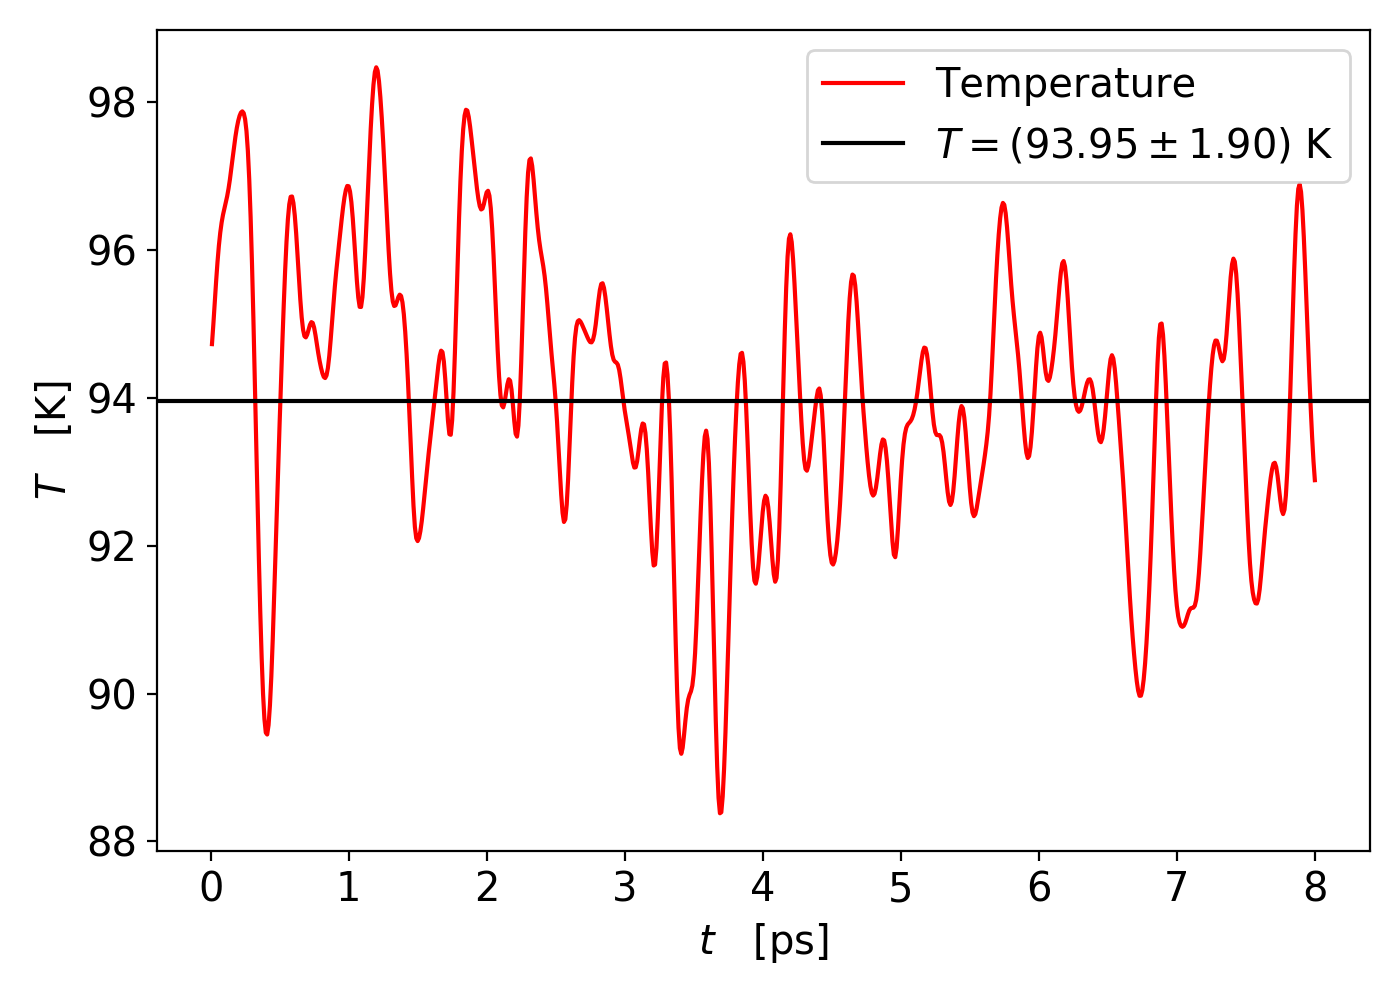
\includegraphics[width=0.99\linewidth]{../task2/results/Tvst}
	\caption{Temperature of the stabilized system in the Grid integration (GI) simulation.}
	\label{fig:Tvst}
\end{figure}
\subsection{Radial distribution function}
\begin{figure}[t]
	\centering
	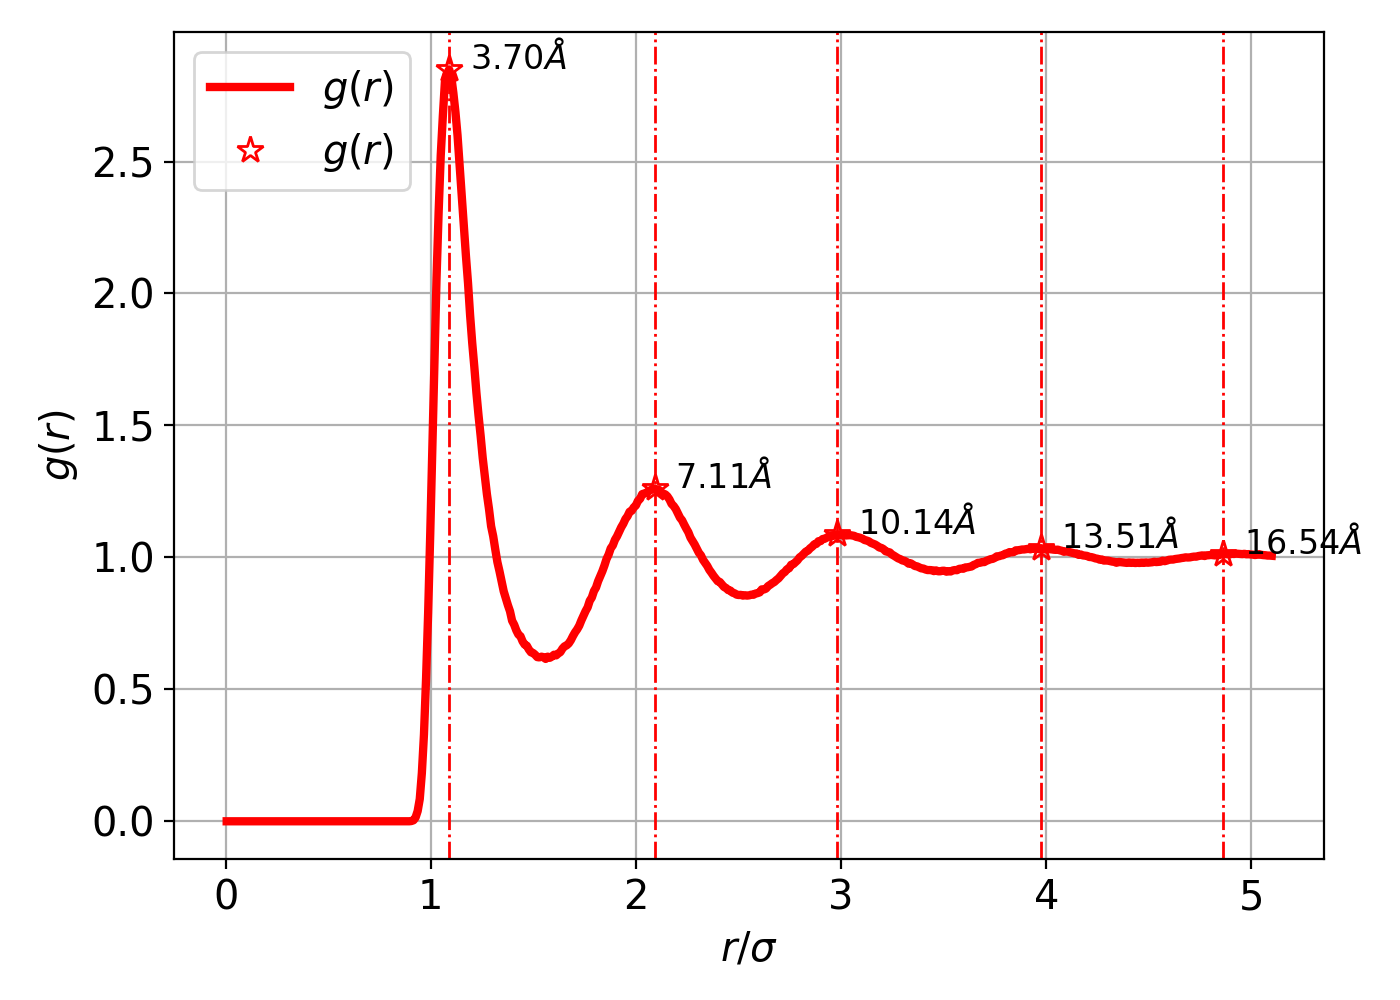
\includegraphics[width=0.99\linewidth]{../task2/results/gofr}
	\caption{Radial distribution function for liquid Argon at $T\approx\SI{94.4}{\kelvin}$ from the GI simulation. The labels on the peaks show the separations $r$ at which it is more likely to find a pair of atoms.}
	\label{fig:gofr}
\end{figure}
\begin{figure}[t]
	\centering
	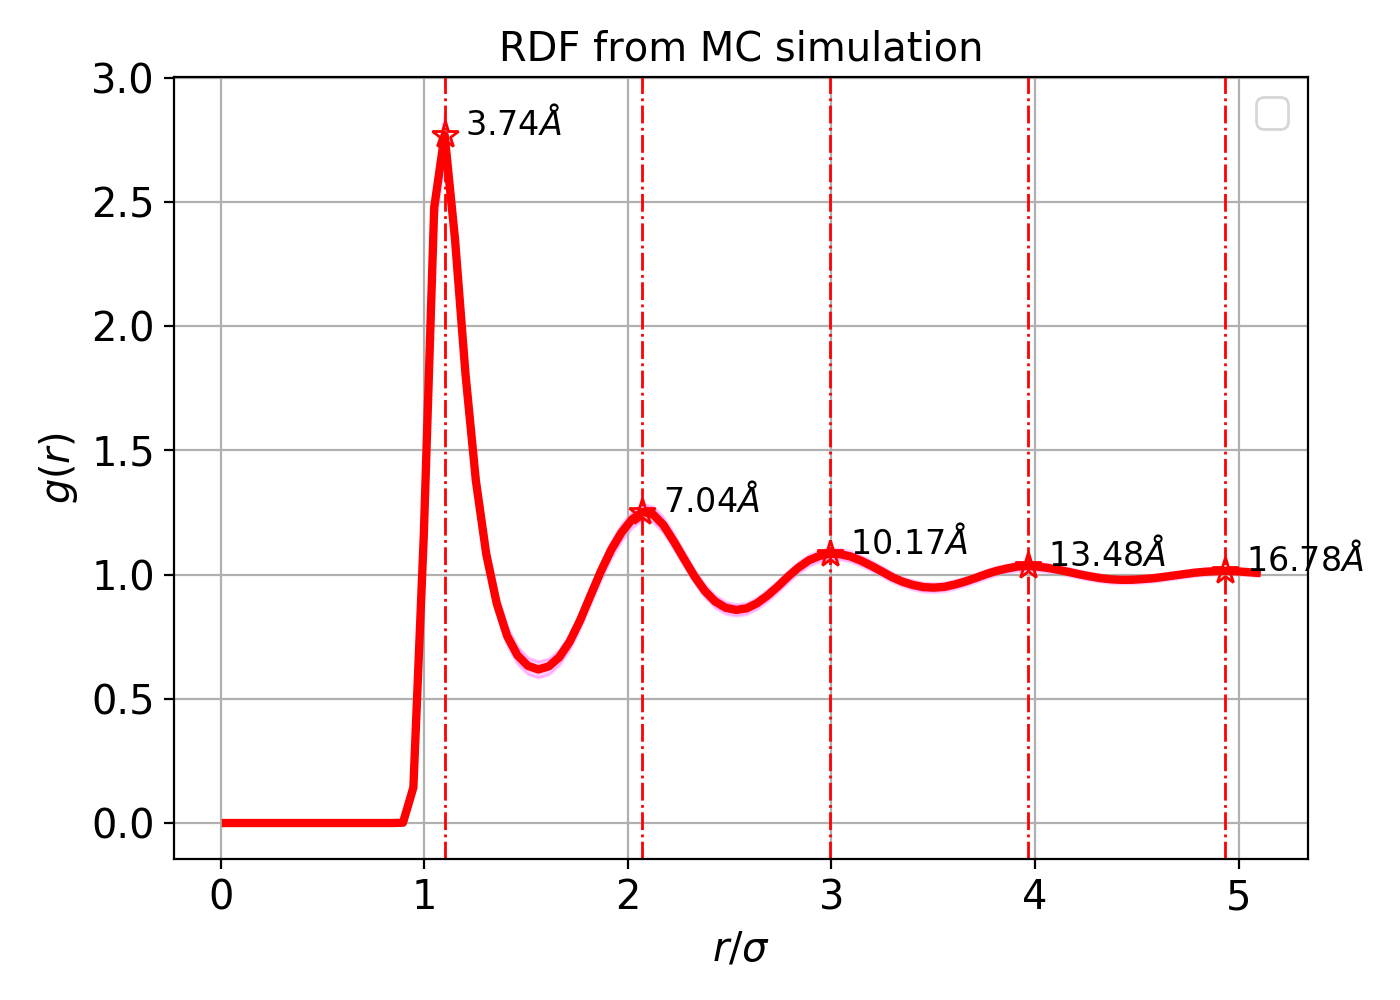
\includegraphics[width=0.99\linewidth]{../task2/results/gofr_mc}
	\caption{Radial distribution function for liquid Argon at $T\approx\SI{94.4}{\kelvin}$ from the MC simulation. The labels on the peaks show the separations $r$ at which it is more likely to find a pair of atoms.}
	\label{fig:gofr_mc}
\end{figure}
The RDF was directly sampled by the \md code and the results are shown in figure \ref{fig:gofr}. The peaks of the curve were extracted  and are also shown (in physical units). The pattern is typical of a liquid, which has no definite crystal structure\cite{Simon2013}. The results are comparable to those shown in \textcite{Rahman1964}, where the first 3 peaks were extracted. The relative errors for these, between the two measurements are $0.10\%,\ 1.58\%$, and $2.59\%$ respectively. Additionally, this simulation allows for the computation of two extra peaks as reported in figure \ref{fig:gofr}.\\
The Monte Carlo simulation is also able to directly sample the RDF at run-time. The number of equilibration and production cycles was set to $\num{100000}$ and the number of steps between property sampling to 5. Figure \ref{fig:gofr_mc} shows the resulting curve. Notice that the curve is indeed very similar to figure \ref{fig:gofr}. The peaks are also shown. These are compared with Ref. \cite{Rahman1964}, resulting in percent errors of 1.04\%, 0.61\% and 2.23\% respectively for the first 3 (available) peaks. Regarding the differences between the grid integration and the MC approaches, the RDFs show sub 1\% differences for the first 5 peaks shown, while the last one presents a 1.5\% percent error. This shows the equivalence of both techniques for the calculation of $g(r)$.
\subsection{Structure factor}
\begin{figure}
	\centering
	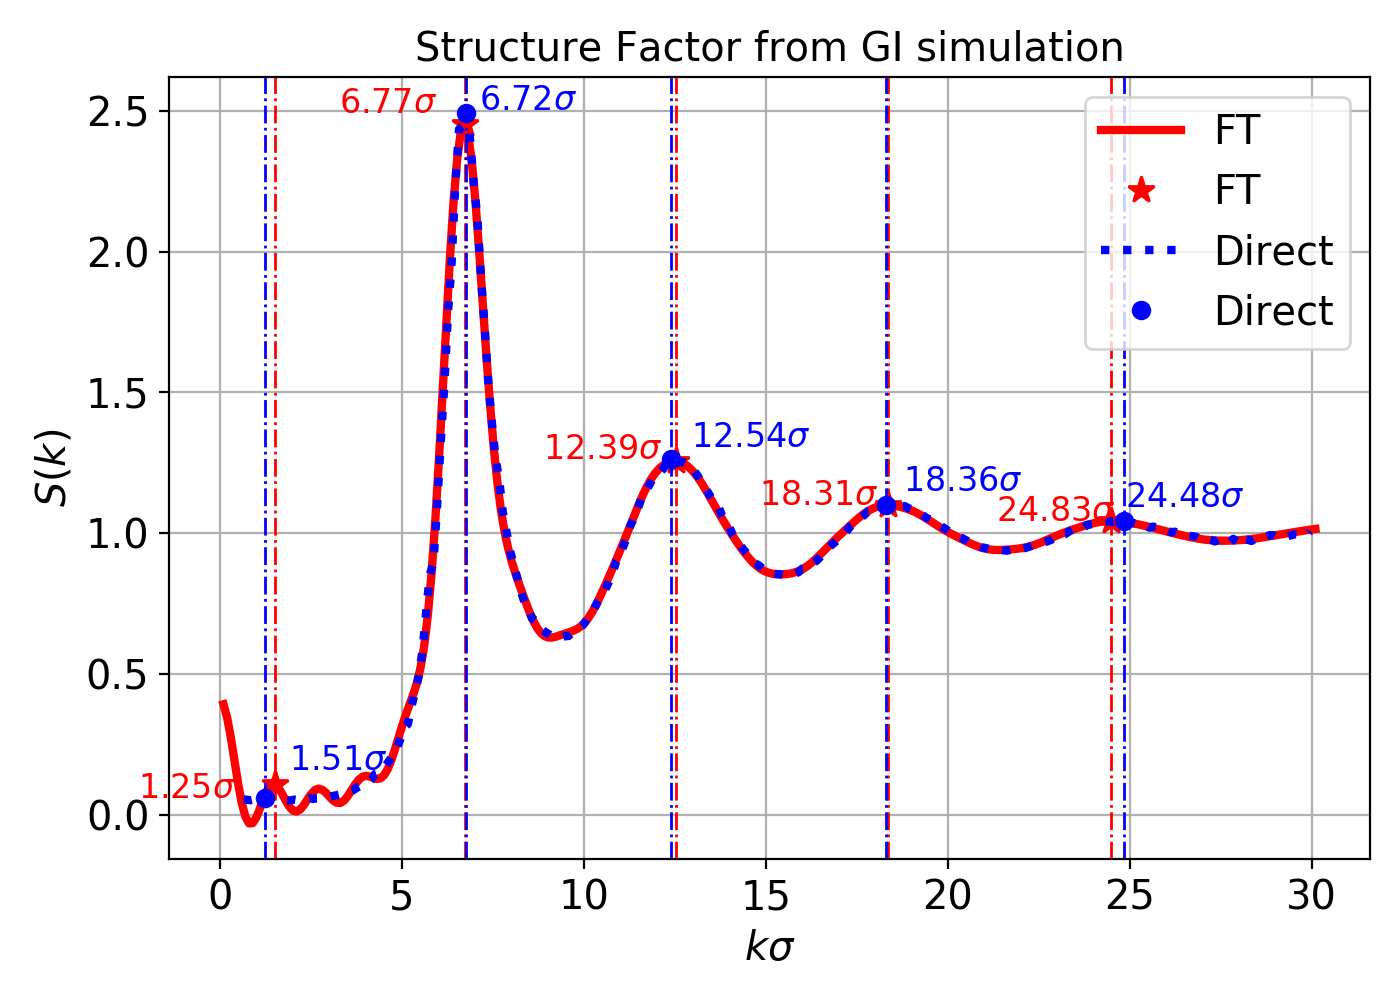
\includegraphics[width=0.99\linewidth]{../task2/results/sofk}
	\caption{Structure factor of liquid Argon at $T\approx\SI{94.4}{\kelvin}$. The values of the peak positions are shown. The values left of the peaks correspond to the FT of $g(r)$ (solid curve), while the values to the right are the peak positions for the directly-sampled curve (dotted line). The first peak is a numerical artifact, we ignore it in this analysis.}
	\label{fig:sofk}
\end{figure}
\begin{figure}
	\centering
	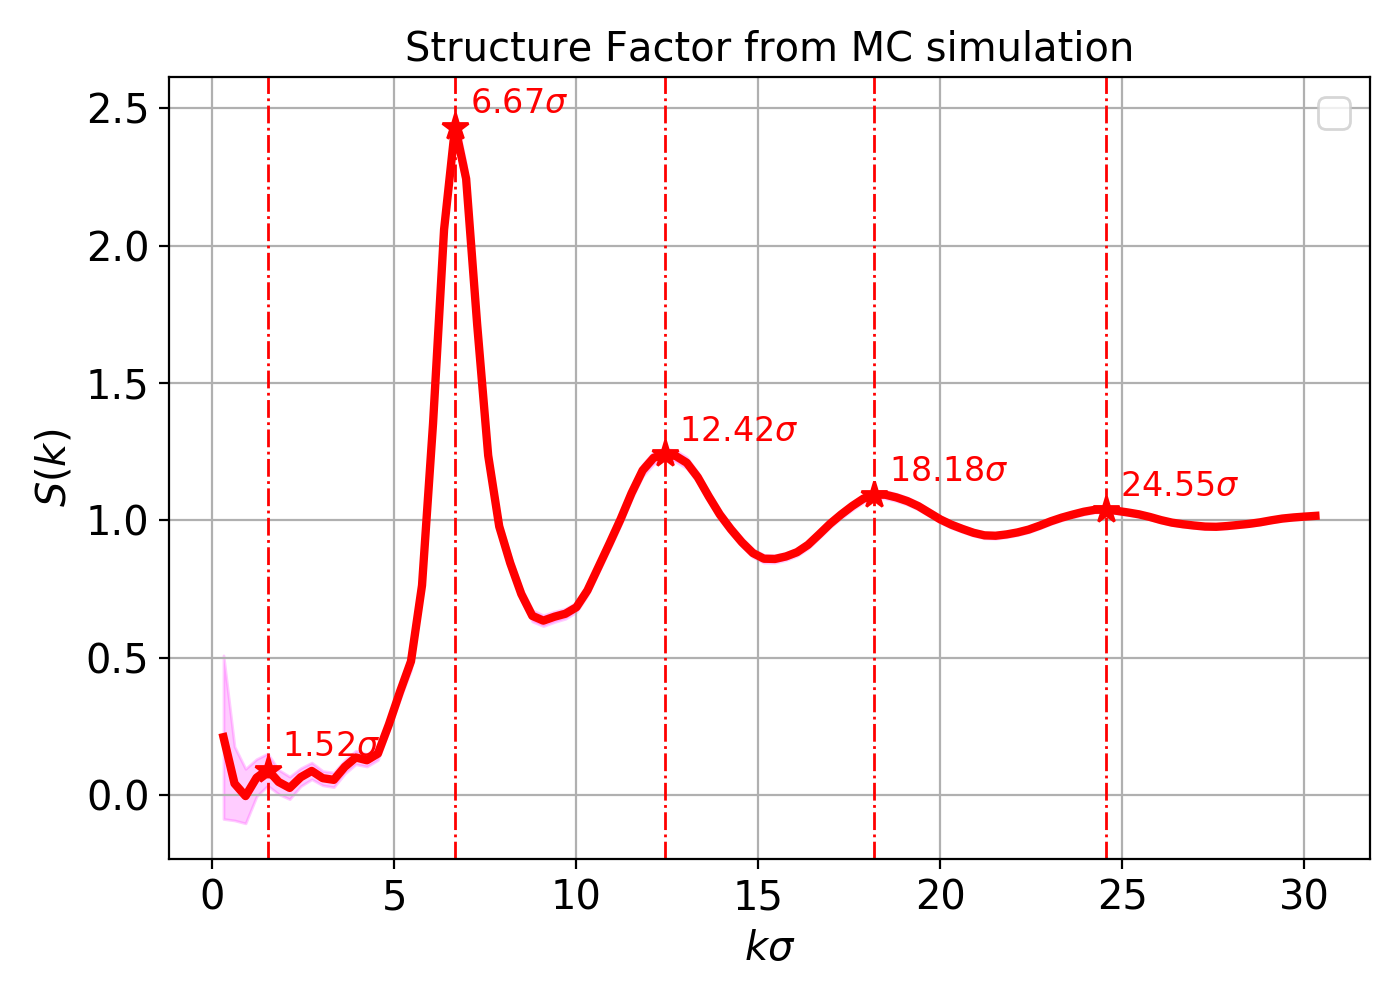
\includegraphics[width=0.99\linewidth]{../task2/results/sofk_mc}
	\caption{Structure factor of liquid Argon at $T\approx\SI{94.4}{\kelvin}$. The values of the peak positions are shown. The shaded region corresponds to the standard deviation of the tries used while the solid line is the mean. The first peak is a numerical artifact, we ignore it in this analysis.}
	\label{fig:sofk_mc}
\end{figure}
The structure factor can either be directly sampled from the velocity distribution or computed as the Fourier transform (FT) of $g(r)$ as shown in equation \ref{eq:sofk}. Both these approaches were taken and results are shown in figure \ref{fig:sofk}. The peak positions are extracted for both cases and are shown in the same figure. The first peak shown has no physical meaning and is more prominent on the FT, given the inaccuracies that arise from this computation. We then focus on the subsequent maxima. The values at the left of each peak in figure \ref{fig:sofk} show the peak positions for the FT computation, while the values on the right show it for the direct sampling case.\\
The values reported in \citet{Rahman1964} are shown in table \ref{tab:sofk} alongside the percent errors for all the approaches tested in the present work. Notice that the errors are relatively small, as in the case of $g(r)$. Furthermore, the average error among all peaks is lowest for the direct sampling case vs. \citet{Rahman1964} (0.61~\%), while the highest is for the MC vs. the same reference (1.3~\%). The last two columns of table \ref{tab:sofk} show the percent errors of the peaks extracted from $S(k)$ sampled from the MC simulation compared to the two techniques used in the GI one. Evidently, the errors are small and, in average, below 1\%. It is then safe to state that the approaches are all equivalent, as expected.\\
It is worth noting that in figures \ref{fig:gofr_mc} and \ref{fig:sofk_mc}, the shaded region corresponding to the ``tries'' or the different extractions of the functions at different steps is almost invisible. Indeed, in the case of $S(k)$, it is only visible in the region of $k\sigma$ close to 0, where the function is dominated by artifacts of the Fourier transform (peaks related to the inverse length of the simulation box). This shows this properties are in fact, static.
\begin{table}
\begin{tabular}{rrrrrr}
	\hline
	$(k\sigma)_{\mathrm{R}}$ &   \% e$_{\mathrm{R-FT}}$ &   \% e$_{\mathrm{R-D}}$ &   \% e$_{\mathrm{R-MC}}$ &   \% e$_{\mathrm{D-MC}}$ &   \% e$_{\mathrm{FT-MC}}$ \\
	\hline
	6.80 &                     1.15 &                    0.40 &                     2.00 &                     1.59 &                      0.84 \\
	12.50 &                     0.33 &                    0.88 &                     0.61 &                     0.27 &                      0.95 \\
	18.50 &                     0.76 &                    1.03 &                     1.75 &                     0.71 &                      0.99 \\
	24.80 &                     1.30 &                    0.13 &                     1.04 &                     1.17 &                      0.26 \\
	\hline
\end{tabular}

\caption{\label{tab:sofk}Values reported for the simulation in reference \cite{Rahman1964} along with the relative percent errors , \%e, among the different measurements. ``R'' represents \citet{Rahman1964}, ``FT'' stands for Fourier transform, ``D'' for direct sampling and ``MC'' for MC direct sampling.}
\end{table}

\subsection{Diffusion Coefficient}
The diffusion coefficient can be computed in two different ways as described in section \ref{sec:diffcoeff}. The first approach is to use de Einstein relation (eq. \ref{eq:diffeinstein}) and compute $D$ from the slope of the MSD. The reported value is the mean of the fitted values to 19 different measurements with their respective standard deviation, $D_{\mathrm{MSD}} = \SI{2.56 \pm 0.24 e-5}{\square\centi\meter\per\second}$. The MSD fit was done starting from $t = \SI{0.3}{\pico\second}$, from where we assumed the ballistic regime had passed, to a relation $\mathrm{MSD(t)}  = \average{\norm{\Delta\vb{r}(t)}^2}= mt + c$. Notice that errors in the fit parameters $m,\ c$ are negligible, thus not reported here in favor of the statistical error in $D_{\mathrm{MSD}}$.\\
\begin{figure}
	\centering
	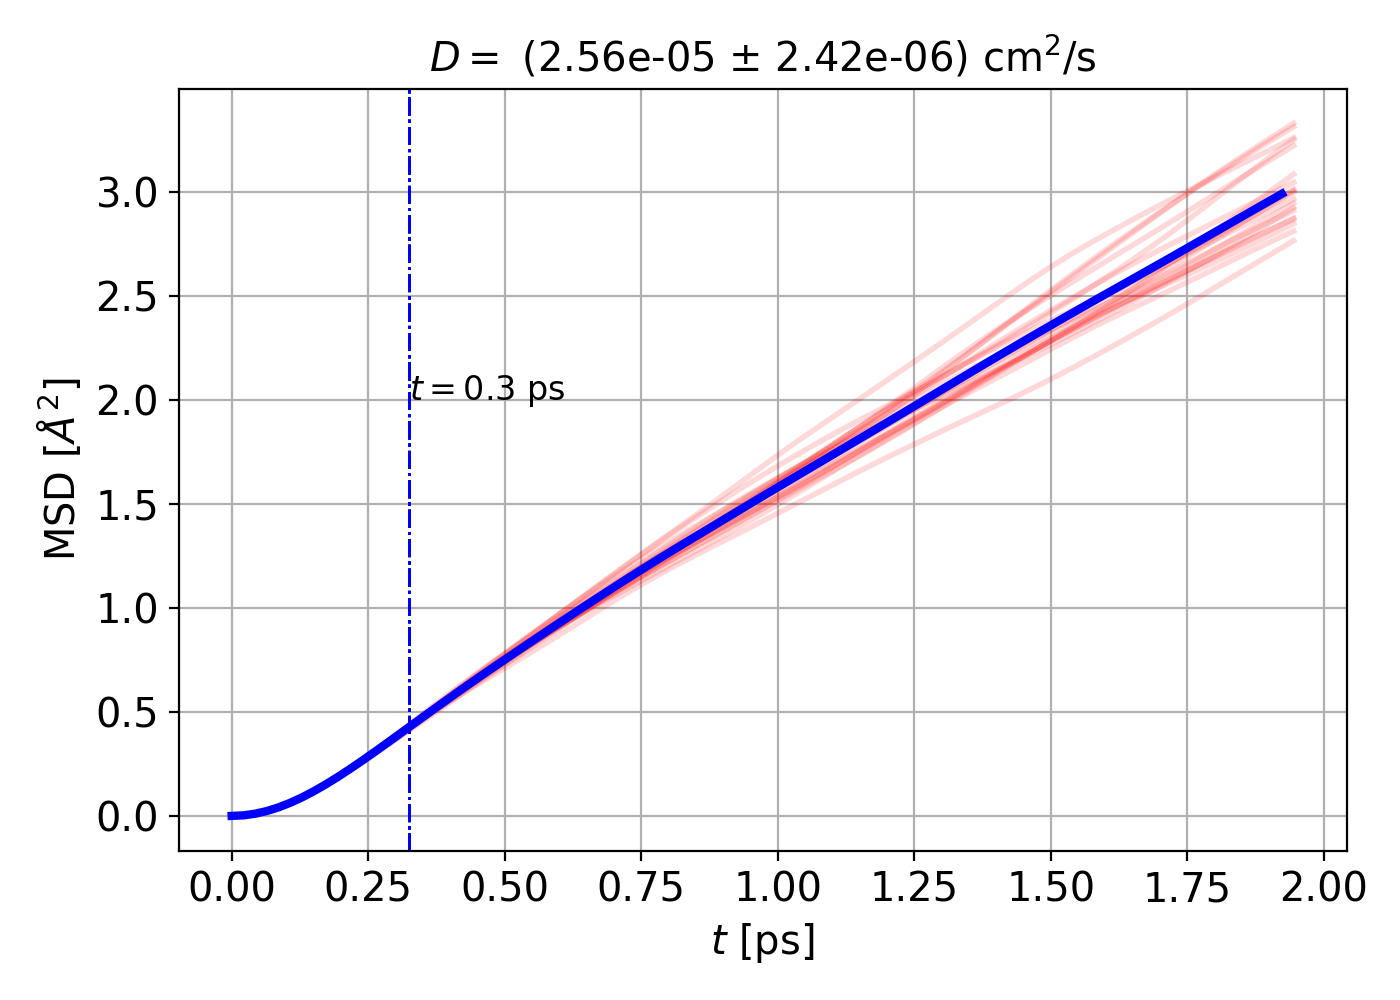
\includegraphics[width=0.99\linewidth]{../task2/results/msdvst}
	\caption{Mean Square Displacement (MSD) obtained from the simulations. The faint (red) lines correspond to each one of the 19 different simulations while the solid (blue) line shows the mean. The vertical line at $t = \SI{0.3}{\pico\second}$ shows the point from which the curves were fitted.}
	\label{fig:msdvst}
\end{figure}
As a second approach, the diffusion coefficient is also calculated from the integral of the VACF. The integral is done numerically with a simple trapezoidal-rule algorithm. The reported value is again the mean of 19 repetitions alongside the respective standard deviation, $D_\mathrm{VACF} = \SI{2,57 \pm 0.3 e-5}{\square\centi\meter\per\second}$. The VACF is shown in figure \ref{fig:vacfvst}.\\
\begin{figure}
	\centering
	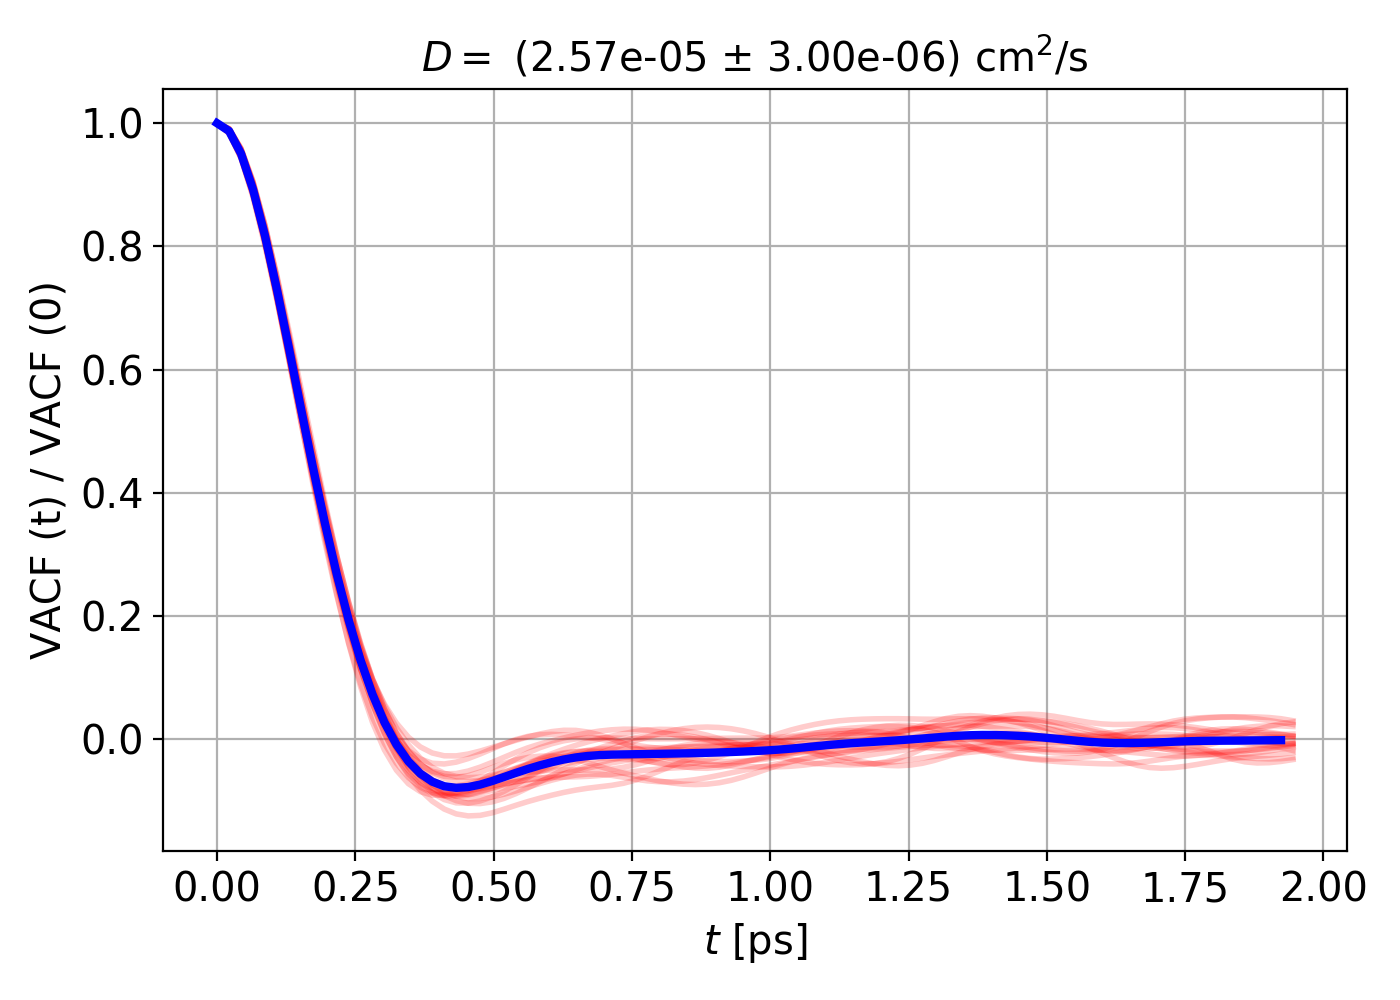
\includegraphics[width=0.99\linewidth]{../task2/results/vacfvst}
	\caption{Normalized VACF plot for the GI simulation. Solid curve shows the mean value of all tries (the 19 simulatons) and the reported value is its integral. Shaded region (faint curves) show the different tries. The reported uncertainty in $D_\mathrm{VACF}$ is given by the standard deviation of the integrals of these curves.}
	\label{fig:vacfvst}
\end{figure}
Evidently, both measured values lie within a single standard deviation from one another. To properly test the agreement between the values, we perform a (different variance) $t$-test with the null hypothesis that the mean values obtained from the slope of the MSD and the integral of the VACF are identical. Such a test yields a $p=0.91 > 0.05$, so we conclude that we can't reject the null hypothesis hence the averages are identical.\\
We can also compare with the results in \citep{Rahman1964}. In this case, we get a $5.31\%$ error in the VACF measurement while in the MSD measurement a value of $4.97\%$ is obtained. In this case we notice that both our values lie below the result in Ref. \cite{Rahman1964}.
\subsection{Blocking Analysis}
In addition to the sampling of $g(r)$ and $S(k)$ from the MC simulation, the energy $E$ and pressure $P$ were obtained from the simulation. During testing, we observed that after $\num{7000}$ cycles, the energy was already stabilized, therefore, the next run was done with $\num{1e6}$ cycles and the equilibration ones were skipped. With these results, 18 block-transformations were applied.\\ Results for the errors in the estimation of $E = \average{H}$ is shown in figure \ref{fig:blockanalysis}. The analysis allows for the computation of the error in $E$ from the plateau value of the curve. This value is taken to be the mean of the last three values in figure \ref{fig:blockanalysis}. The measured value of the energy is then $E = \SI{-95743.47 \pm 7.95e-25}{\joule}$.\\
\begin{figure}
	\centering
	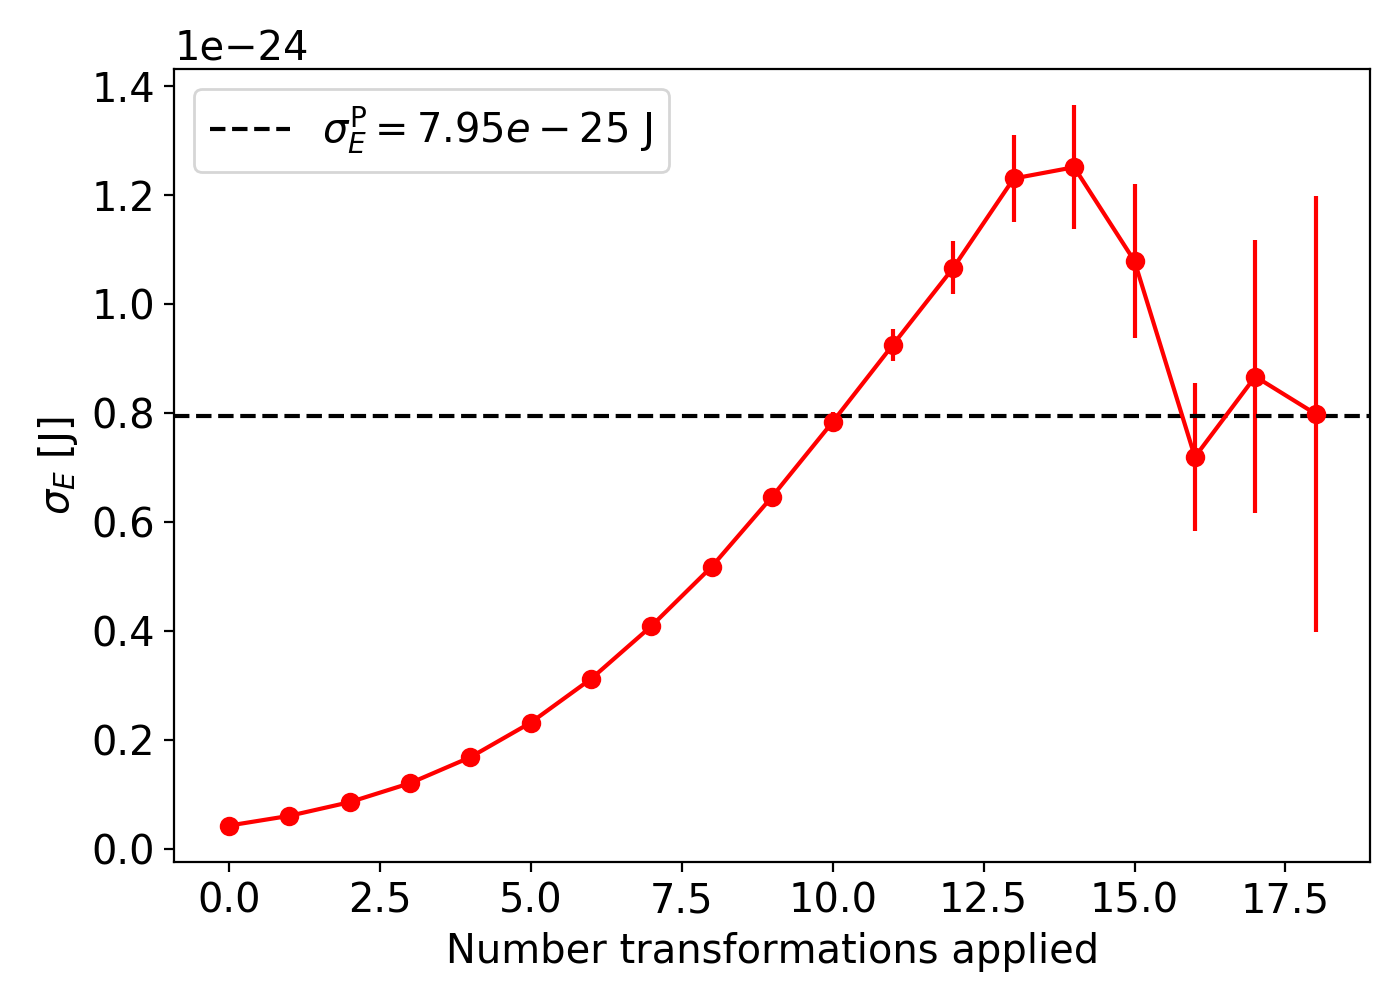
\includegraphics[width=0.999\linewidth]{../task2/results/block_analysis}
	\caption{Results of blocking analysis for the error in the estimation of energy $E$ of the system. Shows the evolution of the uncertainty in the average as a function of the number of transformations applied, $M$ (or equivalently, the block size, $2^M$). The dashed line shows the estimated plateau value.}
	\label{fig:blockanalysis}
\end{figure}
Notice that up to pool 12, $\sigma_E(M)$ was dominated by the exponential factor $2^M$ coming from $N(M)$. However, later it decreases for the next few pools until it starts oscillating around the reported plateau value $\sigma_E^\mathrm{P}$.

\section{Conclusions\label{sec:conclusions}}
We conclude that both simulations show equivalent results in terms of the physical properties of the system that were measured, this is, the static properties $g(r)$ and $S(k)$. Even though both simulations involve integration, the conceptual basis is different. While the GI simulation integrates the equation of motion in configuration space, the MC simulation explores the phase space and finds there the ``physical'' configurations, those with high canonical probability.\\
The features measured have been compared with the results reported in \citet{Rahman1964}. An excellent ($<5\%$) agreement was found in all measurements, validating the present work's results and showing the equivalence between the approaches taken to analyze the system.\\
The GI simulation also allowed us to explore the diffusion coefficient and to compute it in two ways as described before. The values obtained $D_\mathrm{VACF} = \SI{2,57 \pm 0.3e-5}{\square\centi\meter\per\second}$ and $D_{\mathrm{MSD}} = \SI{2.56 \pm 0.24 e-5}{\square\centi\meter\per\second}$ are in agreement as proven by the $t$-test.\\
The error estimation in the MC case for the average energy $E$ was successfully done with blocking analysis, from which a plateau value $\sigma_E^\mathrm{P} = \SI{7.95e-25}{\joule}$ was extracted. We expect a longer simulation would result in a much clearer plateau, however the number of transformations $M$ is very limited by the length of the initial chain $N$. A small increase in $M$ implies an exponential increase in $N$, and thus, in the computing time needed.



\bibliography{refs}
	

\end{document}
%
% ****** End of file aipsamp.tex ******
